\section{Program Logic for Location Virtualization}
\label{sec:logic}
% The predicate gen_heap_interp.
\newcommand{\gammaPred}{\delta}
\newcommand{\gammaPreds}{\delta\textsf{s}}
\newcommand{\rtv}{\textsf{rtv}}
\newcommand{\qone}{\texttt{q1}}
\newcommand{\qtwo}{\texttt{q2}}
\newcommand{\qthree}{\texttt{q3}}
\newcommand{\qfour}{\texttt{q4}}

\newcommand{\sumwalkabs}[3]{
  \ownGhost\gammaPred{\authfrag{\singletonMap{#1}{(#2, #3)}}}
}

\newcommand{\sumapaces}[2]{
  \ownGhost\gammaPreds{\authfrag{\singletonMap{#1}{#2}}}
}
\newcommand{\ptableabswalk}[1]{\mathcal{A}\textsf{bsPTableWalk}(#1)}
\newcommand{\ptablestore}{\theta}

We derive a program logic (a separation logic) supporting the following stances and constraints:
\begin{enumerate}
\item \textit{address-spaces as modal contexts}: Assertions in our logic are context-dependent,
  in the sense that their truth depends on which address space they are used in, due to the need to support virtual points-to assertions.
\item \textit{sharing}: The physical location backing a virtual address's storage is located (during a page table walk) through a 
      set of physical page-table (L4-L1 page-tables) acceses that are shared amongst different virtual addresses (specifically,
      those on the same page of memory\footnote{of in the case of L2 or higher levels of tables, within a given broader region.}).
      This sharing imposes constraints on definiting points-to assertions
      in terms of physical (L4-L1) page-table memory accesses
\item \textit{context-agnostic-resources}: each virtual address is valid under a certain address-space, 
      but it does not represent this \textit{knowledge} of its address-space. 
      That is, assertions are not explicitly tagged with their address space validity
\item \textit{updating address-space mappings}: We present logical abstractions to enable 
      updating not only pages of typical data in memory, but also page tables themselves.\footnote{Prior work relied on unfolding operational semantics
      to verify page table updates.}
\item \textit{explicitly-modal assertions}: Our logic includes a means to talk about facts being true
      in another address space
\item \textit{address-space switch as changing the "World" of truth}: Switching from one address-space to another logically
      becomes a simultaneous introduction-and-elimination of a pair of modal assertions (for different address spaces)
\end{enumerate}

The first viewpoint, that the truth of an assertion is relative to an address space, has far-reaching consequences.
Therefore, as a first step, we work entirely in a pointwise lifting of Iris's base BI logic,
essentially working with separation logic assertions indexed by a page table root as a $\mathcal{W}_{64}$
(Figure \ref{fig:vprop}), which we call $\textsf{vProp }\Sigma$; this is the (\textsc{Coq}) type of assertions in our logic.
Most constructs in Iris's base logic are defined with respect to any BI-algebra (of \textsc{Coq} type \lstinline|bi|), so automatically
carry over to our derived logic.
However, be must still build up from existing Iris primitives to provide new primitives that depend on the address space --- primarily the notion
of virtual points-to.

\begin{figure}[t]
\begin{lstlisting}[language=Coq]
  Definition vProp  $\Sigma$ : bi := word 64 -b> iPropI  $\Sigma$.
  \end{lstlisting}
\caption{$\textsf{vProp }\Sigma$: Root-Address Indexed Address-Space Proposition}
  \label{fig:vprop}
\end{figure}
%\subsection{Machine State under Address Translation}
%\label{sec:selectedinstrsemantics}
%Althought we give the complete set of operational semantics rule in \sref{appendix:movops}, It is worth building the intuition on the the way some of these rules bahave in the context of address translation. In fact $\readlval\maddr{\storememstar\crval}\locsf$ is unfoled into multiple physical memory lookups for the final page address retrieval -- i.e. address translation traversal as shown in Figure \ref{fig:pagetables}:
%\begin{itemize}
%\item top-level-address translation: with the given root address (64-bit $\crval$) of the address space, performs the address translation, handling the first level (to get the PML4 entry) itself. The next level table address is computed with the fetched PML4 offset value which exhibits itself as 9-bit offset in $\kw{maddr}$. \mytodo{iso: put move}
%\item translating from PML4 entry: performs the second level of address translation, to retrieve starting at the PML4 table entry, and interprets the PML4 entry that references a Page-Directory-Pointer Table (PDPT). We obtain the PDPT offset which exhibits itself as 9 bit offset in $\kw{maddr}$ to obtain the address of the next level page directory table (PDT) \mytodo{iso: put move}
%\item translating from PD entry: performs the third level of address translation, to retrieve starting at the PDP table entry, and interprets a PDPTE that references a PD table. Likewise, we obtain the PD offset which exhibits itself as 9 bit offset in $\kw{maddr}$ to obtain the address of the next level page directory table (PT) \mytodo{iso:put move }
%\item translate from PT entry: performs final level of address translation, starting from the PT entry, with a given 12 bit page offset, we can compute the physical address referencing $\locsf$ \mytodo{ismo: put mov}
%\end{itemize}

\subsection{Base Points-To Assertions}
\label{sec:pointsto}
We build up our context-dependent assertions from two basic types of assertions that do not care about address spaces.
% We abstract physical memory addressing and registers naming with well-known separation logic assertion \textit{points-to} assertions.
% \begin{enumerate}
% \item Physical address points-to, $\pfpointsto\locsf\vpts\qfrac\ppts$
% \todo[inline,color=red]{Colin says: This syntax is what most readers would expect for physical poinst-tos, but it's
% inconsistent with the split 52+12  stuff later... Whatever we do, we need to be consistent}
% \item Register points-to, $\pfpointsto\rg\rv\qfrac\rpts$
% \end{enumerate}

\paragraph{Register points-to} 
The assertion $\pfpointsto\rg\rv\rpts\qfrac$ ensures the ownership of the register $\rg$ naming the register value $\rv$. 
The fraction $\qfrac$ with value 1 asserts the unique ownership of the register mapping, and grants update permission on it, 
otherwise, any value $0 < \qfrac <1$ represents partial ownership granting readonly permission on the mapping.

\paragraph{Physical memory  points-to} The soundness proofs for our logic's rules largely center around page-table-walk accesses as in Figure \ref{fig:coq_addr_translation},
 where (inside the helper functions) we need to split a 64-bit word representing entries in these tables into 52-bit segments
which specify the physical page number of another page in the walk, and 12-bit segments containing various control bits.
For this reason we have two notions of physical points-to facts. The primitive notion closest to our machine model is:
\[ \textsf{w1} \ \sim \ \textsf{w2} \mapsto_{\textsf{a}} \; \{\textsf{q}\} \; \textsf{v} \]
In this form, we see that \textsf{w1} (a $\mathcal{W}_{52}$) essentially selects a 4KB page of physical memory,
and \textsf{w2} (a $\mathcal{W}_{12}$) is an offset within that page.
% could be an 52-bits masked address to level 4 table 
% ($\textsf{w1 } =( \textsf{ l4M52 maddr cr3val}) $),
%and, expectedly \textsf{w2} is an address computed by page-offset computation (e.g. $\textsf{l4off maddr cr3val}$). 
From this we can derive a more concise physical points-to when the split is unimportant:
% Giving a raw 64-bits memory pointsto assertion becomes
\[\textsf{w} \mapsto_{\textsf{p}} \{q\} \textsf{ v} \stackrel{\triangle}{=} (\textsf{drop 12}~w) \ \sim \ (\textsf{bottom 12}~w)\mapsto_{\textsf{a}} \textsf{ v} \]

\begin{figure*}
  \begin{lstlisting}[language=Coq]
 Definition $\vaddr\mapsto_{\textsf{t}}\{\textsf{q}\}\; \vpage$ : vProp $\Sigma$ := 
  $\exists_{\textsf{l4e l3e l2e l1}} \ldotp$  $\ulcorner$ aligned $\vaddr \urcorner \ast$ L4_L1_PointsTo(maddr l4e l3e l2e l1e) $\ast$ addr_L1$(\vaddr,\textsf{l1e}) \mapsto_{p}\{\mathsf{q}\} \vpage$.
 Definition L4_L1_PointsTo (maddr l4e l3e l2e l1e :word 64) : vProp $\Sigma$ :=
 $\lambda$ cr3val.
  $\ulcorner$ entry_present l4e $\land$ entry_present l3e $\land$ entry_present l2e $\land$ entry_present l1e$\urcorner$ $\ast$
  (l4M52 maddr cr3val) $\sim$ (l4off maddr cr3val) $\mapsto_{a}$ {q1}  l4e  $\ast$
  (l3M52 maddr l4e) $\sim$ (l3off maddr l4e)  $\mapsto_{a}$ {q2}  l3e $\ast$ 
  (l2M52 maddr l3e) $\sim$ (l2off maddr l3e) $\mapsto_{a}$ {q3}  l2e $\ast$
  (l1M52 maddr l2e) $\sim$ (l1off maddr l2e) $\mapsto_{a}$ {q4}  l1e.
\end{lstlisting}
\vspace{-1em}
\caption{A Strong Virtual Points-to Relation}
\todo[inline,color=red]{Colin, I updated the definition with entry present}
  \label{fig:strongvirtualpointsto}
\end{figure*}



\subsection{An Overly-Restrictive Definition for Virtual Memory Addressing}
\label{sec:overly-restrictive}
A natural definition for a virtual points-to that depends on the current address space is to
require that in order for a virtual address \textsf{va} to point to a value \textsf{v}, the assertion contains
partial ownership of the physical memory involved in the page table walk that would translate \textsf{va} to
its backing physical location --- with locations existentially quantified since a virtual points-to should not assert
\emph{which} locations are accessed in a page table walk.
Figure \ref{figure:strongvirtualpointsto} gives such a definition.
It asserts the existence of for page table entries, one at each translation level, and via \lstinline|L4_L1_PointsTo|
asserts from the current \lstinline|cr3| value, taking the offsets from \textsf{va} (as in Figure \ref{fig:pagetables})
to index each level, finding the existentially quantified entries in each level, 
ending with the L1 entry, whose physical page base is added to the page offset of \textsf{va} to obtain the physical address
 --- and there (\lstinline|addr_L1(va,l1e)|) in physical memory, is the value.
Most of the definition lives directly in \textsf{vProp}, using the separation logic structure lifted from Iris's \textsf{iProp}.

\lstinline|L4_L1_PointsTo| works by
chaining together the entries for each level, using the sequence of table offsets from the address being translated to index
each table level, and using the physical page address embedded in each entry.
For example, 
  the first level address translation to get the L4 entry (\lstinline|l4e|) 
  uses the masks \textsf{l4M52} with the current \lstinline|cr3| to get the 
  physical address of the start of the L4 table,
  and \textsf{l4off} with the virtual address being translated to compute the correct offset within that table.
  Then at that physical location is the appropriate entry in the L4 table \textsf{l4e}.
  Subsequent levels of the page table walk work similarly.
The statement of these assertions is simplified by the use of our split physical points-to assertions, since
each level of tables is page-sized.\footnote{We do not address superpages and hugepages in this paper.}
This helper definition is also a more explicit \textsf{vProp}, explicitly binding a value for \lstinline|cr3| and using it
to start the translation process.


% Given the definition of physical page-pointsto assertion and the root address of virtual-address space as shown in Figure \ref{fig:pagetable}, one can build the physical address-translation for a virtual address (e.g. \textsf{va}) via abstracting the L4-L1 table traversal as the following:
% \begin{itemize}
%   \item Level-4 Translation (L4): Performs 
%   the first level address translation to get the L4 entry (L4E) in Figure \ref{fig:pagetables} by using the masks l4M52 and l4off with \textsf{rtv} virtual base address to get the starting address of the L4 table (L4T), and locate the entry amongst 512 (q1) ones respectively.
%     \begin{lstlisting}[language=Coq]
%       $\hbox{(\TirNameStyle{{L4translate}})} \quad$ (l4M52 maddr rtv) \$\sim$\ (l4off maddr rtv) $\mapsto_{a}$ {q1} l4e 
%     \end{lstlisting}
%  \item Level-3 Translation (L3): Performs the second level address translation to get the L3 entry (L3E) in Figure \ref{fig:pagetables} by using the masks l3M52 and l3off with L4 entry (l4e) to get the starting address of the L3 table (L3T), and locate the entry amongst 512 ones (q2) respectively.
%     \begin{lstlisting}[language=Coq]
%     $\hbox{(\TirNameStyle{{L3translate}})}$ (l3M52 maddr l4e) \$\sim$\ (l3off maddr l4e)  $\mapsto_{a}$ {q2} l3e
%     \end{lstlisting}
%   \item Level-2 Translation (L2): Performs the second level address translation to get the L2 entry (L2E) in Figure \ref{fig:pagetables} by using the masks l2M52 and l2off with L3 entry (l3e) to get the starting address of the L2 table (L2T), and locate the entry amongst 512 ones (q3) respectively.
% \begin{lstlisting}[language=Coq]
%     $\hbox{(\TirNameStyle{{L2translate}})}$ (l2M52 maddr l3e) \$\sim$\ (l2off maddr l3e)  $\mapsto_{a}$ {q3} l2e
%     \end{lstlisting}
%   \item Level-1 Translation (L1): Performs the second level address translation to get the L1 entry (L1E) in Figure \ref{fig:pagetables} by using the masks l1M52 and l1off with L2 entry (l2e) to get the starting address of the L1 table (L1T), and locate the entry amongst ones 512 (q4) respectively.
%    \begin{lstlisting}[language=Coq]
%     $\hbox{(\TirNameStyle{{L1translate}})}$ (l1M52 maddr l2e) \$\sim$\ (l1off maddr l2e)  $\mapsto_{a}$ {q4} l1e
%     \end{lstlisting}
%   \item Page Address Level Translation: Final computed physical page-address ($\textsf{addr\_L1}(\vaddr$,$\textsf{l1e}$)) points-to the value stored in the address ($\vpage$).
%    \begin{lstlisting}[language=Coq]
%     $\hbox{(\TirNameStyle{{PageLevelAccess}})} \qquad$ addr_L1($\vaddr,\textsf{l1e}$) $\mapsto_{p} \vpage$.
%     \end{lstlisting} 
% \end{itemize}

This solution is in fact very close to that of \citet{kolanski08vstte}, who define a separation logic from scratch in \textsc{Isabelle/HOL},
where the semantics of all assertions are functions from pairs of heaps and page table root values to booleans.\footnote{
  This was a typical explicit construction at the time; their work significantly predates Iris.
}
Our solution removes some restrictions in this definition by further abstracting the handling of address translation.

\subsection{Aliasing/Sharing Physical Pages}
  \label{sec:sharingpages}  
  One might have already observed that the virtual points-to definition shown in Figure \ref{fig:strongvirtualpointsto} 
  is too strong to specify some operations a virtual memory manager may need to do, such as
  move one level of the page table to a different physical location while preserving all virtual-to-physical mappings.\footnote{
    x86-64 hardware, like other architectures, includes a feature (which we do not formalize assertions for) to
    replace an L1 page table address in an L2 entry with a pointer to a \emph{larger} 2MB page (called super-pages), 
    or replace an L2 page table address in an L3 entry with a pointer to a 1GB page (called huge-pages).
  }
   To speak more concretely, the fractional permissions on the page-table-walk assertion ($\textsf{L}_{4}\_\textsf{L}_{1}\_\textsf{PointsTo}$ in Figure \ref{fig:strongvirtualpointsto}) 
  ensure fractional ownership of the four physical page table entries accessed by the hardware during address translation,
  as well as the physical memory holding the data of the virtual points-to.
  However, this formulation stores knowledge of the page table walk's details with ownership of the backing physical
  memory.
  Updating any of these mappings (e.g., moving the page tables in physical memory, as in coallescing for
  superpages or hugepages)
  would require explicitly collecting all virtual points-to facts that traverse affected entries.
  It is preferable to permit the page tables themselves to be updated independently of the virtual points-to assertions,
  so long as those updates preserve the same virtual-to-physical translations.
\newcommand{\vale}{\textsf{val}}
\begin{figure*}
\[
\begin{array}{l}
    \vaddr\mapsto_{\textsf{v}}\{\textsf{q}\}\vale : \mathsf{vProp}~\Sigma \stackrel{\triangle}{=} \\
    \quad
    \exists \paddr\ldotp
    \exists \delta\ldotp
    \underbrace{\lambda\mathit{cr3val}\ldotp\sumapaces{\mathit{cr3val}}\delta}_\text{\begin{tabular}{c}Find ghost map for this\\address space\end{tabular}} \ast 
  \underbrace{\sumwalkabs\vaddr\qfrac\paddr }_\text{\begin{tabular}{c}Fractional ownership of \\virt-to-phys translation\end{tabular}}\ast 
  \underbrace{\paddr \mapsto_{\mathsf{p}} \vale}_\text{\begin{tabular}{c}Value at\\physical location\end{tabular}}
\end{array}
\]
\caption{Virtual-Pointsto for Sharing Pages}
  \label{fig:virtualpointstosharing}
\end{figure*}  

  Intuitively, the definition in Figure \ref{fig:strongvirtualpointsto} is too strong because the virtual points-to
  assertion there tracks too much information: when writing programs that access memory via virtual addresses,
  most code does not care \emph{which physical memory locations are involved in address translation}: it only cares
  that virtual address translation would succeed. The necessary information about the physical page table walk
  must still be tracked, but can be tracked separately from the virtual points-to assertion itself.

  We take the approach of separating the physical page-table-walk pointsto ($\textsf{L}_{4}\_\textsf{L}_{1}\_\textsf{PointsTo}$ in Figure \ref{fig:strongvirtualpointsto}) 
  from the virtual pointsto relation. 
  To do so, we take advantage of an Iris construction which permits tracking a map in ghost state that maps
  virtual addresses to the physical addresses they translate to, and has for each key in the map (i.e.,
  each virtual address) a token. Updating the virtual-to-physical (ghost) mapping for a virtual address $va$
  requires full ownership of the token. In addition, we keep an invariant that for each $va\mapsto pa$ mapping
  in this map, there are \emph{physical} resources sufficient to ensure that address translation for $va$
  will resolve in the hardware to $pa$. But these physical resources, which specify \emph{which} physical locations
  are involved in the page table walk, are now separated from but consistent with
  the knowledge that such resources exist (which is embodied by the token for $va$, which tracks that $va$ maps to $pa$
  in the ghost map). Thus we can store the token which summarizes the translation and ensures it exists in the virtual
  points-to, and keep the ghost map and the invariant that every mapping in the ghost map has corresponding physical resources
  for translation in a separate global invariant.

  % To do so, we introduce the protocol separating read-only (fragmental) and authorative (full ownership) accesses to the page tables, specifically $\textsf{L}_{4}\_\textsf{L}_{1}\_\textsf{PointsTo}$. 
  % We realize this protocol by embedding it into an already existing \textsf{Iris}'s ghost-map (or view\_maps) construction
  In Iris this is realized by using an authoritative resource algebra: there is a single \emph{authoritative} global copy of the (ghost)
  map caching virtual-to-physical address translations, and for each entry a read only \emph{partial} ownership of that key-value pair.
  The resource algebra itself is instantiated as:
  \[\mathcal{A}\textsf{bsPTableWalk} \stackrel{\triangle}{=} \textsc{Auth} (\; \mathcal{W}_{64} \;\rightarrow_{\textrm{fin}} \;  ( (\textsc{Frac }, \mathord{+}) \times (\textsc{Agree } \Loc,\mathord{=}) ))\]
We replace the physical
 $\textsf{L}_{4}\_\textsf{L}_{1}\_\textsf{PointsTo}$
with
fragmental ownership of the ghost-map ($ \sumwalkabs\vaddr\qfrac\paddr$),
 whose ownership just ensures that the virtual address ($\vaddr$) is mapped to a page (referenced by $\paddr$)


We place the authorative ownership $\mathcal{A}\textsf{PTableWalk}$ of the ghost-map in a per-address-space invariant
($\mathcal{I}$\textsf{ASpace} in Figure \ref{fig:peraspaceinvariant}) whose ownership, when combined with the
fraction stored in the virtual points-to, permits changes in the virtual-to-physical translations.
By itself, it allows changes to the page tables as long as they do not change the overall mappings from virtual
to physical addresses.



  \begin{figure*}
\[
\begin{array}{l}
  \mathcal{I}\textsf{ASpace}(\ptablestore,m)\stackrel{\triangle}{=} \textsf{ASpace\_Lookup}(\ptablestore,m) \ast \\
 \qquad\qquad\qquad \bigast{(\vaddr, \textsf{l1e})\in \ptablestore}{\exists\;(\textsf{l4e l3e l2e})\ldotp \textsf{L}_{4}\_\textsf{L}_{1}\_\textsf{PointsTo}(\textsf{ maddr, l4e, l3e, l2e, l1e})} \\
  \textsf{ where } \\
   \textsf{ASpace\_Lookup} (\ptablestore,m) \stackrel{\triangle}{=} \lambda\textsf{ cr3val} \ldotp \; \exists \gammaPred \; \ldotp \ulcorner m \; !!\; \textsf{cr3val} = \textsf{Some } \gammaPred \urcorner \ast
    \ownGhost\gammaPred{\authfull{\ptableabswalk\ptablestore}}
  
\end{array}
\]
\caption{Global Address-Space Invariant with a fixed global map of address-space names $m$}
  \label{fig:peraspaceinvariant}
  \end{figure*}

Another major change is that, because our logic is the first to explicitly address the existence of multiple address spaces,
the ghost map of virtual-to-physical translations (identified by the ghost name $\delta$ in Figure \ref{fig:virtualpointstosharing}
 \emph{for each address space}. This means we also require a way to locate the map for the current address space
from the current root page table pointer stored in \lstinline|cr3|.

Figure \ref{fig:peraspaceinvariant} describes the resources for each address space, which are collected
for the full address space, but separated from virtual points-to assertions.
$\Theta$ is the logical map from virtual addresses to the physical addresses they should translate to, 
for the \emph{current} address space, corresponding to the currently installed page tables (the ones
indicated by \lstinline|cr3|). In Figure \ref{fig:virtualpointstosharing}, the existentially-quantified $\delta$
is the ghost name for the authoritative copy of this map (again, for the current address space).
$m$ is the (full) logical map from the various page table bases to ghost names for the 
per-address-space mappings like $\Theta$.
It is the full version of the map named by the ghost name $\delta{}s$ in
Figure \ref{fig:virtualpointstosharing}; there is only one such map in the system.
This is why Figure \ref{fig:virtualpointstosharing} asserts there is some ghost name in that (global) map
for the current address space.
The global map itself is tracked by a resource algebra 
\[\mathcal{A}\textsf{spaces} \stackrel{\triangle}{=} \textsc{Auth} (\; \mathcal{W}_{64} \;\rightarrow_{\textrm{fin}} \;  ( (\textsc{Frac }, \mathord{+}) \times (\textsc{Agree } \Loc,\mathord{=}) )) \]
\todo[inline]{shouldn't above be map to gname, not these pairs?}


$\mathcal{I}\textsf{ASpace}(\Theta,m)$ is then the resources for the current address space:
It ensures that the current address space is valid (it has an entry in $m$, whose corresponding
authoritative map matches $\Theta$), and asserts ownership of the appropriate fractional ownership
of the physical page table walk for each virtual-to-physical translation in $\Theta$ (for the current address space).



  
Figure \ref{fig:logicaladdrspace} depicts the relationships between these pieces, for a single
address space.
The invariant for the currently active address space (solid round square labelled as 
$\mathcal{I}$\textsf{ASpace} in Figure \ref{fig:logicaladdrspace}) asserts authorative ownership (i.e. 
update capability), $\ownGhost\gammaPred{\authfull{\ptableabswalk\ptablestore}}$, of the ghost map $\Theta$
describing virtual-to-physical address translations
-- shown as a solid-round-head arrow to $\mathcal{A}\textsf{PTableWalk}$.
Each virtual points-to assertion (dashed round square labelled as \textsf{Virtual PointsTo}
 in Figure \ref{fig:peraspaceinvariant})
asserts fragmental ownership of the ghost map $\Theta$, $\sumwalkabs\vaddr\qfrac\paddr$,
shown via the dashed-diamond-head arrow to $\mathcal{A}\textsf{PTableWalk}$. Specifically, it asserts that
the virtual address the virtual points-to assertion concerns corresponds to some physical address.
There exists only one persistent authorative ownership 
($\ownGhost\gammaPred{\authfull{\ptableabswalk\ptablestore}}$) which collects the fragmental 
ghost page-table-walk mapping ($\sumwalkabs\vaddr\qfrac\paddr$),
 shown as double-ended solid arrow 1 to N imposing the update protocol.

\begin{figure}
   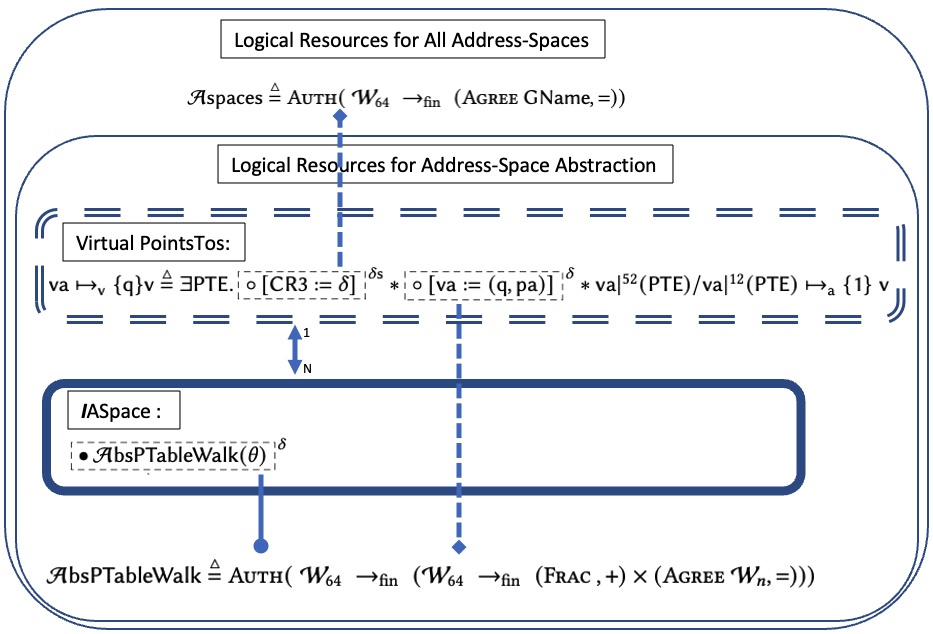
\includegraphics[width=0.75\columnwidth]{logical_addr_space.png}
  \caption{Logical Resources of Address-Space Abstraction (1 Address Space)}
  \label{fig:logicaladdrspace}
  \end{figure}

\paragraph{From A Single Address Space to Many}
In principle the resources from each individual address space should be collected into a single
shared invariant, and for each memory access,
a fragment of this corresponding to $\mathcal{I}\textsf{ASpace}(\Theta,m)$
for the current address space should be extracted from this global resource, used to prove correctness of the
memory access, and put back.
In this paper we focus on the middle section, explicity identifying resources for each
address space. The reason for this is that in practice, this global resource is also
the place where kernel-specific assumptions, such as guaranteeing that certain virtual address range
was mapped in all address spaces, would be enforced. This paper focuses on the
reasoning principles behind the virtual memory access, and we leave the use of this within a larger
kernel to future work.

\subsection{Address-Space Management}
\label{sec:aspacemanagement}
So far, we have introduced logical abstractions for a single address space. However, virtual memory management
implementations typically handle more than one address-space,
and doing this requires assertions which talk about other address spaces, and means to switch address spaces.
% requiring a means to  which we abstract as a ghost map from root address of an address-space to a namespace labelling the address space

% \paragraph{Valid Context-Resources} Fragmental ownership of $\mathcal{A}\textsf{spaces}$ ($\sumapaces\rtv\gammaPred$) conveys the fact that a current address-space ($\gammaPred$) is the one selected, i.e. loaded into the $\rtv$. This simple fact becomes essential when we observe it inside virtual-pointsto definition in Figure \ref{fig:virtualpointstosharing} and pictorially Figure \ref{logicaladdrspace}. Existence of this fragmental ownership ensures that the contextual resource, i.e. a virtual pointsto assertion, resides under the correct address-space, i.e. modal-context, that makes it valid.

% \paragraph{Modal Resource Context\&Interaction with Ambient Logic \textsf{vProp}}
% \label{sec:resourcecontext}
% The relation between the address-space and and the validity of virtual-pointsto assertions exhibits itself as a contingency, i.e. \textit{"a certain virtual-pointsto facts whose validity is indexed by the root address of an address space"}. But, what sort of convenience this pattern provides when we do reasoning about more than one address-space.

% In Figure \ref{fig:addrswitch}, we see two different address-spaces rooted at R0 and R1 in the pre/post condition. To be put into words, while switching an address-space by executing \lstinline|mov_ctl|) updating the  \lstinline|cr3|, it is expected to mention resources of two different address-spaces in the specification. In the precondition,  \lstinline|cr3| is loaded with R0 and all the virtual-pointsto assertions $a_0 \mapsto_{\textsf{v}}p_0$ and $a_1 \mapsto_{\textsf{v}}p_1$ are in the current-view of the memory and valid in the ambient logic \textsf{vProp}. The other address-space with the root address R1 has its own resources ($b_0 \mapsto_{\textsf{v}}p_3$ and $b_1 \mapsto_{\textsf{v}}p_4$) which are invalid under the current address space rooted at R0. This pattern of specification requires resources being mentioned under the \textit{world} they are valid, i.e. a modal-framing within the specification. Once the current address-space becomes the one with root address R1, i.e.  \lstinline|cr3| is loaded with R1, the context-resources $b_0 \mapsto_{\textsf{v}}p_3$ and $b_1 \mapsto_{\textsf{v}}p_4$ are loaded into the current-view of the memory, and all the other resources that are valid under R0 are introduced into the modal context rooted at R0
\begin{figure}
\[
  \begin{array}{r@{\qquad}l}
    \hbox{(\TirNameStyle{ModalAddressSpace})} &
         [r](\mathsf{P}) \;: \mathsf{vProp} \; \Sigma \; \stackrel{\triangle}{=} \; \lambda \_,\; \mathsf{P}~\mathsf{r}.\\
    \hbox{(\TirNameStyle{ModalAddressSpaceMono})} & (\textsf{P} \vdash \textsf{Q}) \vdash  ([r](\textsf{P}) \vdash  [r](\textsf{Q}))\\
    \hbox{(\TirNameStyle{ModalAddressSpaceSep})} & [r](\textsf{P} \ast \textsf{Q}) \dashv\vdash ([r](\textsf{P}) \ast [r](\textsf{Q})\\
    \hbox{(\TirNameStyle{ModalAddressSpaceAnd})} &   [r](\textsf{P}\land \textsf{Q}) \dashv\vdash [r](\textsf{P})\land [r](\textsf{Q})\\    
    \hbox{(\TirNameStyle{ModalAddressSpaceOr})} &    [r](\textsf{P}\lor \textsf{Q}) \dashv\vdash [r](\textsf{P})\lor [r](\textsf{Q})\\   
    % \hbox{(\TirNameStyle{ModalAddressSpacePure})} &  \textsf{pure\_vprop P}(\textsf{iPropI }\Sigma)\textsf{ : vProp }\Sigma \stackrel{\triangle}{=} \; \lambda \_ \ldotp \textsf{P}\\
    \hbox{(\TirNameStyle{ModalAddressSpaceFact})} &  \textsf{Fact P} \stackrel{\triangle}{=} \;\forall \; ,r \; r' \ldotp  \textsf{P r} \dashv\vdash \textsf{P r'}\\
    % \hbox{(\TirNameStyle{ModalAddressSpaceFactIntroElim})} \\
    % \qquad\qquad \textsf{Fact pure\_vprop P} \vdash  ([r](\textsf{pure\_vprop P}) \dashv\vdash (\textsf{pure\_vprop P}) (\textsf{vProp }\Sigma))\\
    \hbox{(\TirNameStyle{ModalAddressSpaceFactIntroElim})} 
    &\textsf{Fact P} \vdash  ([r](\textsf{P}) \dashv\vdash (\textsf{P}) %(\textsf{vProp }\Sigma))\\
  \end{array}
  \]
  \caption{Other-space Modality and Its Laws}
  \label{fig:modaldef}
  \end{figure}
Figure \ref{fig:modaldef} gives the definition of our modal operator for asserting truth of a modal
(address-space-contingent) assertion \emph{in another address space}, which we call
the \emph{other-space} modality. The definition itself is not
particularly surprising --- as our modal assertions are semantically predicates on a page table root (physical)
address, the assertion $[r](P)$ is a modal assertion which ignores the (implicit) current page table root,
and evaluates the truth of $P$ as if $r$ were the page table root. This simple definition is first of all
enough for assertions in one address space to talk about assertions in another.

More usefully, we can prove that this modality follows certain useful laws, and that it interacts with
a class of assertions which are true regardless of which address space they are evaluated in.
The other-space modality distributes over the various separation logic connectives, and follows the rule of
consequence.
We also define a class of \textsf{vProp}s we call \textsf{Fact}s, which are those assertions
which ignore their address space entirely.
Physical points-tos and register value assertions, when treated as \textsf{vProp}s, are \textsf{Fact}s.
\textsf{Fact}s can move in and out of other-space modalities freely.


  
\begin{figure}
\[
\begin{array}{l}
  \{ \textsf{cr3 } \mapsto_{r} R0 \ast a_0 \mapsto_{\textsf{v}}p_0  \ast a_1 \mapsto_{\textsf{v}}p_1  \ast [r1]\;( b_0 \mapsto_{\textsf{v}}p_3  \ast b_1 \mapsto_{\textsf{v}}p_4 )\}\\
  \qquad \qquad \qquad \qquad \qquad \mathsf{mov\_ctl} \;\; \texttt{cr3} \; \; R1\\

  \{ \textsf{cr3 } \mapsto_{r} R1 \ast [r0](a_0 \mapsto_{\textsf{v}}p_0  \ast a_1 \mapsto_{\textsf{v}}p_1)  \ast  b_0 \mapsto_{\textsf{v}}p_3  \ast b_1 \mapsto_{\textsf{v}}p_4 \}
  \end{array}
\]
  \label{fig:addrswitch}
  \end{figure}

\begin{remark}[The Choice of Modal Context, Contingency and  Pattern of Verification Context]
  \label{remark:pattern}
The truth on an address space, exhibits itself as a contingent truth: a location virtualization assertion (a virtual points-to in \ref{fig:virtualpointstosharing}),  happens to valid in the \textit{current world} (in the current address space), and switching address spaces pulls information out of one \textit{world} into the “current view” of memory, and leaves other assertions true relative to the previous address space.

Therefore, an address-space, as an abstraction, can be treated as naming the memory state as a modal frame and the choice of page table root as a world in Kripke-style semantics. Not suprisingly, transition between two address-spaces, then, can be just an entailment relation \textit{alternating} the \textit{named-state}

Being inspired by what hybrid logic \ref{} calls a satisfaction operator, which evaluates the truth of a predicate in a named alternative state (here, address space), we give a modal definition describing the truth of assertions for the resources (i.e. virtual pointsto relations) inside the address space. Ignoring the predicate types for a while, $[r]P$ in Figure \ref{fig:modaldef}, indicates that $P$ holds in the virtual address space rooted at $r$, the truth ($P$) on an address-space is indexed by the root page-table address $r$ of the address-space. In the rest of this section, we explain the structural aspects -- the modal resource context of address space modality -- , and how we lift the interaction of address-space modality with the ambient logic, i.e. separation logic as an entailment for specifying \textit{address-space-switch}.

Pragmatically, 
  \begin{enumerate}
  \item a modal context with its context-resources and picked contingency defines a modality (e.g. a address-space modality $[r]P$). For the convenience of verification, it enables focusing on the certain facts in the interest of reasoning (e.g. virtual pointsto relations in the current address-space)
  \item and, offloads the burden of individual bookkeeping of these facts (e.g. virtual pointsto relations per address-space) under different context (e.g. virtual pointsto relations in other address-spaces) via utilizing the \textit{summarization} aspect of the contingency it represents (e.g. other virtual pointsto relations are valid under other certain address-space page-table root addresseses).  
  \end{enumerate}
\end{remark}

\subsection{The Impact of Changing Address Spaces on Modal Assertions}
% \subsection{Considering Hoare Doubles in the Context of Switching Address-Space}
% \subsubsection{Issues with Using Hoare Triples in Address-Space Specification}
\label{sec:issues}
An important subtlety arises with supporting \lstinline|mov|s into \lstinline|%cr3|. Consider the hypothetical rule:
\begin{mathpar}
\inferrule[Broken]{ }{
  \{P \ast \textsf{cr3}\mapsto_{r} \;r_1 \ast r \mapsto_{r} \;r_2 \ast [r_2](Q)\}
  \texttt{mov}~\texttt{\%cr3},~r%\lstinline|mov %cr3, r| 
  \{[r_1](P) \ast \textsf{cr3} \mapsto_{r} r_2 \ast r \mapsto_{r} r_2 \ast Q\}
}
\end{mathpar}
This rule captures the intuitive change of address space in a Hoare triple.
The problem with this is that it interacts quite poorly with the traditional frame
rule and the modal flavor of virtual points-to assertions.
If we abbreviate the pre- and post-conditions above as \textsf{Pre} and \textsf{Post}:
\begin{mathpar}
  \inferrule*[right=Frame]{
    \inferrule*[right=Broken]{ }{
    \{\textsf{Pre}\}
    \texttt{mov}~\texttt{\%cr3},~r%\lstinline|mov %cr3, r| 
    \{\textsf{Post}\}
    }
  }{
    \{a\mapsto_\mathsf{v} x \ast \textsf{Pre}\}
    \texttt{mov}~\texttt{\%cr3},~r%\lstinline|mov %cr3, r| 
    \{a\mapsto_\mathsf{v} x \ast \textsf{Post}\}
  }
\end{mathpar}
Notice that both the precondition and postcondition assert that $a\mapsto_\mathsf{v} x$ in the current address space, but we have no basis for concluding that address translation is preserved by the change of address space. So this derivation clearly leads to an unsound conclusion. 
This suggestss that the traditional frame rule and the Hoare triple presentation of the change-of-address-space rule cannot soundly coexist in the same system.
The heart of the problem is that while updating \lstinline|cr3| is \emph{physically} local, it globally changes the interpretation of virtual addresses. So it is simply unsound to frame around \lstinline|cr3| updates.
In hindsight this is not surprising, because we have essentially defined
our assertions to depend on resources they do not explicitly mention --- the value of \lstinline|cr3|.
However, it has important impacts on our formal development.

\todo[inline]{Colin revision frontier}

Switching to Hoare doubles resolves this problem because an under-appreciated subtlety of Hoare doubles is that typically \emph{there is no frame rule}. Instead each verification essentially includes a local frame that it passes to the next instructions (think continuation-passing style), giving each overall rule a \emph{global} (rather than local) precondition. For most rules this is not that important, but it does permit rules that have global effects on their preconditions.

This is then how we justify our actual rule for \lstinline|cr3| updates:
\begin{mathpar}
\inferrule[ChangeAddressSpace]{
  \{[r_1](P) \ast cr3 \mapsto_{r} r_2 \ast r \mapsto_{r} r_2 \ast Q\}\overline{is}
}{
  \{P \ast cr3 \mapsto_{r} r_1 \ast r \mapsto_{r} r_2 \ast [r_2](Q)\}
  \texttt{mov}~\texttt{\%cr3},~r;\;\overline{is}
  %\lstinline|mov %cr3, r| 
}
\end{mathpar}
Because the precondition on this rule is global, we avoid issues with framing.

If we wanted to consider a frame rule that would work for this logic, we could consider:
\begin{mathpar}
  \inferrule[Cr3Frame]{
    \{P\ast cr3=v\}\;C\;\{ Q \ast cr3=v\}
  }{
    \{R\ast P\ast cr3=v\}\;C\;\{ R \ast Q \ast cr3=v\}
  }
\end{mathpar}
By demanding that \lstinline|cr3| be held constant (or rather, at least restored to its original value) we could frame almost traditionally. In particular, this rule would work with framing around calls that might lead to address space switches, such as calling blocking operations in the kernel.

Readers familiar with dynamic frames~\cite{parkinson2011relationship} might find it useful to notice that a different perspective on this matter is that virtual points-to assertions are self-stable \emph{except} for changes in \lstinline|cr3|, so framing would then naturally require other means of holding \lstinline|cr3| constant (or saving and restoring it).
Virtual points-to assertions could be made self-stable by also giving them partial ownership over \lstinline|cr3| assertions, but this would require explicitly plumbing that ownership from \emph{all} assertions back to any place an address space change might occur; this would seem to be a far graver loss of modularity than this extra quirk in framing discussions.
\subsection{Selected Logical Rules}
\label{sec:selected_rules}
Based on the issues we discuss in Section \ref{sec:issues}, we make sure our Hoare-Double definition in Figure \ref{fig:wpddefinition} enables
\begin{itemize}
\item virtual-pointsto relations to be independent of \lstinline{cr3} ownership
\item and full-ownership of \lstinline to be propagated inside the \textsf{wpd\_def} in order to
\end{itemize}
This act of separation allows client-specification to be agnostic of \lstinline|cr3| physical resource, (i.e. \lstinline|cr3| $\mapsto_{\textsf{r}} \rtv$). The context-resource (virtual-pointsto) has only the \textit{knowledge} of being in a namespace in which it is valid ($\sumapaces\rtv\gammaPred$), nothing more.

In the rest of this, we explain how specifications of some selected \textsf{AMD64} instructions look like under the decisions made on the reasoning principles. All rules, e.g. the ones with different addressing mode, can be found in our artifact.

In the general outline of the proof in Figure \ref{wpdamd}, we see that each rule annotated with an address value (\textsf{rtv}), i.e. a root address of an address-space, under which the resources mentioned in the specification are valid. Moreover, there is a frame resource $P$ in each rule.
\begin{figure} 
  \[
  \begin{array}{l}
    \textsf{wpd\_def e s E1 } \Phi \;\mathsf{ rtv } : \textsf{iProp }\Sigma := \\
   \qquad ((\textsf{cr cr3}) \mapsto_{\textsf{r}} (\textsf{num rtv)}) \textsf{ rtv}) \ast (\Phi \textsf{ rtv}) \wand \textsf{WP e E } @ \textsf{s ; E1 } \{\{\_, \textsf{True} \}\}
    \end{array}
  \]
\caption{Unfolded Hoare-Double Definition for \textsf{vProp} Logic }
\label{fig:wpddefinition}
\end{figure}

\begin{figure}
\begin{mathpar}
  \inferrule[WriteToRegFromReg]{
  \{P \ast r_d \mapsto_{r} \textsf{rvs} \ast r_s \mapsto_{r}\{q\} \textsf{ rvs} \}_{\textsf{rtv}}\;\overline{ is}
}{
  \{P \ast r_d \mapsto_{r} \textsf{rvd} \ast r_s \mapsto_{r}\{q\} \textsf{ rvs} \}_{\textsf{rtv}}
  \textsf{ mov}~\textsf{r}_d,~\textsf{r}_s;\;\overline{is}
  %\lstinline|mov %cr3, r| 
}
\\
\inferrule[WriteToPhysMemFromReg]{
  \{P \ast r_s \mapsto_{r}\{q\}  \textsf{rvs}  \ast r_a \mapsto_{r} \{q\} \textsf{ vaddr} \ast \textsf{vaddr} \mapsto_{\textsf{t}} \textsf{v} \}_{\textsf{rtv}}\;\overline{ is}  
}{
  \{P \ast r_s \mapsto_{r}\{q\}  \textsf{rvs}   \ast r_a \mapsto_{r}\{q\} \textsf{ vaddr} \ast \textsf{vaddr} \mapsto_{\textsf{t}} \textsf{rvs} \}_{\textsf{rtv}}
  \textsf{ mov}~\textsf{r}_a,~\textsf{r}_s;\;\overline{is}
}
\\
\inferrule[WriteToRegFromPhysMem]{
  \{P \ast r_d \mapsto_{r}  \textsf{v} \ast r_a \mapsto_{r} \{q\} \textsf{ vaddr} \ast \textsf{vaddr} \mapsto_{\textsf{t}} \textsf{v} \}_{\textsf{rtv}}\;\overline{is}
}{
  \{P \ast r_d \mapsto_{r}  \textsf{rvd} \ast r_a \mapsto_{r} \{q\} \textsf{ vaddr} \ast \textsf{vaddr} \mapsto_{\textsf{t}} \textsf{v} \}_{\textsf{rtv}}
  \textsf{mov}~\textsf{r}_d,~\textsf{r}_a;\;\overline{is}
}
\\
\inferrule[WriteToRegFromVirtMem]{
  \{P \ast \mathcal{I}\textsf{ASpace}\ast \mathcal{I}\textsf{ASpace} \ast r_d \mapsto_{r}  \textsf{v} \ast r_a \mapsto_{r} \{q\} \textsf{ vaddr} \ast \textsf{vaddr} \mapsto_{\textsf{v,rtv}} \textsf{v} \}_{\textsf{rtv}}\;\overline{is}
}{
  \{P \ast \mathcal{I}\textsf{ASpace}\ast r_d \mapsto_{r}  \textsf{rvd} \ast r_a \mapsto_{r} \{q\} \textsf{ vaddr} \ast \textsf{vaddr} \mapsto_{\textsf{v}} \textsf{v} \}_{\textsf{rtv}}
  \textsf{mov}~\textsf{r}_d,~\textsf{r}_a;\;\overline{is}
}
\\
\inferrule[WriteToVirtMemFromReg]{
  \{P \ast \mathcal{I}\textsf{ASpace}\ast r_s \mapsto_{r}\{q\}  \textsf{rvs}  \ast r_a \mapsto_{r} \{q\} \textsf{ vaddr} \ast \textsf{vaddr} \mapsto_{\textsf{v}} \textsf{v} \}_{\textsf{rtv}}\;\overline{ is}  
}{
  \{P \ast \mathcal{I}\textsf{ASpace}\ast r_s \mapsto_{r}\{q\}  \textsf{rvs}   \ast r_a \mapsto_{r}\{q\} \textsf{ vaddr} \ast \textsf{vaddr} \mapsto_{\textsf{v}} \textsf{rvs} \}_{\textsf{rtv}}
  \textsf{ mov}~\textsf{r}_a,~\textsf{r}_s;\;\overline{is}
}
\\
\inferrule[WriteToRegCtlFromReg]{
  \{P \ast r_s \mapsto_{r}\{q\}  \textsf{ rvs}  \}_{\textsf{rvs}} \overline{is}
}{
  \{P \ast r_s \mapsto_{r}\{q\}  \textsf{ rvs}   \}_{\textsf{rtv}}
  \textsf{mov}~\textsf{cr3},~r_s;\;\overline{is}
  %\lstinline|mov %cr3, r| 
}\\
\inferrule[WriteToRegFromRegCtl]{
  \{P \ast r_d \mapsto_{r} \textsf{rvs} \ast r_s \mapsto_{r}\{q\} \textsf{ rvs} \}_{\textsf{rtv}}\;\overline{ is}
}{
  \{P \ast r_d \mapsto_{r} \textsf{rvd} \ast r_s \mapsto_{r}\{q\} \textsf{ rvs} \}_{\textsf{rtv}}
  \textsf{ mov}~\textsf{r}_d,~\textsf{r}_s;\;\overline{is}
  %\lstinline|mov %cr3, r| 
}
\end{mathpar}
\caption{Reasoning Rules for Selected \textsf{AMD64} Instructions under}
\label{fig:wpdamd}
\end{figure}
\subsubsection{Memory To Register}
In Figure \ref{fig:wpdamd}, we see the rules for updating the memory address ($r_a$). To do so, we essentially need page-table-walk pointsto ($\textsf{L}_{4}\_\textsf{L}_{1}\_\textsf{PointsTo}$ in Figure \ref{fig:strongvirtualpointsto}) to locate the value to be written. We mainly have two options to achieve this. 
\paragraph{Physical Memory To Register} First one is to use  page-table-walk pointsto ($\textsf{vaddr} \mapsto_{\textsf{t}} \textsf{v}$), which is consists of all-physical page-table memory assertions, to prove the page-table traversal \textsf{AMD64} implements, update the register $r_d$ the value obtained ($\textsf{v}$) as shown in Figure (\TirNameStyle{WriteToRegFromPhysMem}). By doing so, we expose the resources ($\textsf{L}_{4}\_\textsf{L}_{1}\_\textsf{PointsTo}$) needed only for the proof of \textsf{AMD64} page-table traversal to the client of the rule. This breaks the modularity of reasoning we want to maintain in location virtualization.
  \paragraph{Virtual Memory To Register}  Therefore, we would like to use a virtual-pointsto assertion ($\textsf{vaddr} \mapsto_{\textsf{v},\textsf{rtv}}$), which hides physical resources needed for the proof of page-table-traversal from the client, to obtain the the value ($\textsf{v}$) to update the register $r_d$ as shown in Rule (\TirNameStyle{WriteToRegFromVirtMem}). While doing the proof of page-table-traversal with a given virtual-pointsto definition in Figure \ref{fig:virtualpointstosharing}, we unfold and obtain our token ($\sumwalkabs\vaddr\qfrac\paddr$) to exchange for a physical-table mapsto assertion inside the $\mathcal{I}\textsf{ASpace}$ ($\textsf{L}_{4}\_\textsf{L}_{1}\_\textsf{PointsTo}$) in Figure \ref{fig:peraspaceinvariant}, and apply Rule (\TirNameStyle{WriteToRegFromPhysMem}).
\paragraph{Updating \lstinline|cr3|} Unlike other rules, \TirNameStyle{WriteToRegCtlFromReg} updates the root address of the address-space determining the validity of resources, $\{\rtv\} / \{\textsf{rvs}\}$.

